\documentclass[a4paper]{article}
\usepackage[spanish]{babel}
\usepackage[utf8]{inputenc}
\usepackage{charter}   % tipografia
\usepackage{graphicx}
%\usepackage{makeidx}
\usepackage{paralist} %itemize inline
\usepackage{pdfpages}


%\usepackage{float}
%\usepackage{amsmath, amsthm, amssymb}
%\usepackage{amsfonts}
%\usepackage{sectsty}
%\usepackage{charter}
%\usepackage{wrapfig}
%\usepackage{listings}
%\lstset{language=C}


\usepackage{color} % para snipets de codigo coloreados
\usepackage{fancybox}  % para el sbox de los snipets de codigo

\definecolor{litegrey}{gray}{0.94}

% \newenvironment{sidebar}{%
% 	\begin{Sbox}\begin{minipage}{.85\textwidth}}%
% 	{\end{minipage}\end{Sbox}%
% 		\begin{center}\setlength{\fboxsep}{6pt}%
% 		\shadowbox{\TheSbox}\end{center}}
% \newenvironment{warning}{%
% 	\begin{Sbox}\begin{minipage}{.85\textwidth}\sffamily\lite\small\RaggedRight}%
% 	{\end{minipage}\end{Sbox}%
% 		\begin{center}\setlength{\fboxsep}{6pt}%
% 		\colorbox{litegrey}{\TheSbox}\end{center}}

\newenvironment{codesnippet}{%
	\begin{Sbox}\begin{minipage}{\textwidth}\sffamily\small}%
	{\end{minipage}\end{Sbox}%
		\begin{center}%
		\vspace{-0.4cm}\colorbox{litegrey}{\TheSbox}\end{center}\vspace{0.3cm}}



\usepackage{fancyhdr}
\pagestyle{fancy}

%\renewcommand{\chaptermark}[1]{\markboth{#1}{}}
\renewcommand{\sectionmark}[1]{\markright{\thesection\ - #1}}

\fancyhf{}

\fancyhead[LO]{Sección \rightmark} % \thesection\ 
\fancyfoot[LO]{\small{Aldasoro Agustina, Bouz\'on Mar\'ia Bel\'en, Cairo Gustavo Juan}}
\fancyfoot[RO]{\thepage}
\renewcommand{\headrulewidth}{0.5pt}
\renewcommand{\footrulewidth}{0.5pt}
\setlength{\hoffset}{-0.8in}
\setlength{\textwidth}{16cm}
%\setlength{\hoffset}{-1.1cm}
%\setlength{\textwidth}{16cm}
\setlength{\headsep}{0.5cm}
\setlength{\textheight}{25cm}
\setlength{\voffset}{-0.7in}
\setlength{\headwidth}{\textwidth}
\setlength{\headheight}{13.1pt}

\renewcommand{\baselinestretch}{1.1}  % line spacing


% \setcounter{secnumdepth}{2}
\usepackage{underscore}
\usepackage{caratula}
\usepackage{url}




\begin{document}


\thispagestyle{empty}
\materia{M\'etodos Num\'ericos}
\submateria{Segundo Cuatrimestre de 2014}
\titulo{Trabajo Práctico III}
\subtitulo{Develando la mentira de los megap\'ixeles}
\integrante{Aldasoro Agustina}{86/13}{agusaldasoro@gmail.com}
\integrante{Bouz\'on Mar\'ia Bel\'en}{128/13}{belenbouzon@hotmail.com}
\integrante{Cairo Gustavo Juan}{89/13}{gjcairo@gmail.com}

\maketitle
\newpage

\thispagestyle{empty}
\vfill
\begin{abstract}
En el presente trabajo se pretende analizar y comparar distintas alternativas que pretenden dar respuesta al problema de demosaicing. Para ello, las mismas serán implementadas y sometidas a experimentación sobre fotografías crudas sintéticas específicamente seleccionadas para poner de manifiesto las ventajas e inconvenientes del empleo de cada método. \\
\end{abstract}

\textbf{Palabras clave:} \\
$\bullet$ Filtro Bayer \\
$\bullet$ Demosaicing \\
$\bullet$ Interpolaci\'on \\
$\bullet$ Artifacts \\



\thispagestyle{empty}
\vspace{3cm}
\tableofcontents
\newpage


%\normalsize
\newpage

\section{Introducci\'on Te\'orica}

Promediando la década de 1990 comenzaron a introducirse al mercado las cámaras digitales de uso hogareño, empezando a sustituir desde entonces a las ampliamente difundidas cámaras de film. 
Mientras que estas últimas capturaban la imagen de forma mecánica y sin intercesión de un procesamiento digital, las cámaras electrónicas emplearon una nueva tecnología. Esta tecnolog\'ia distingue entre en el momento de obtención de un conjunto de datos cerca del objetivo – donde se obtiene una imagen que llamaremos “\textit{cruda}” – y una etapa de procesamiento automático conjunto a la reconstrucción de la imagen final. \\

En el presente trabajo nos interesará analizar un fragmento de dicha etapa conocido como \emph{demosaicing}. Para entender de qué consta, es menester comprender previamente la forma en que se capturan las imágenes al utilizar cámaras digitales.

Este tipo de cámaras poseen un sensor CCD compuesto de una matriz de elementos fotosensibles, cada uno de los cuales es capaz de captar la intensidad de la luz que llega a ese punto a través de la lente. 

La tarea de capturar todos los colores reflejados por el objetivo que se quiere fotografiar no está encomendada a ninguna posición en particular, sino que cada una de ellas tiene asignada – de acuerdo a algún patrón definido  – la captura de la información perteneciente a un solo color. Cada p\'ixel de la imagen va a estar dividido en tres canales ya que la vamos a almacenar, en nuestro caso de estudio, mediante RGB (Red, Green, Blue).

El patr\'on que determina qué color será capturado por cada fotosensor es denominado \emph{Color Filter Array} y var\'ia de acuerdo al fabricante de c\'amaras. Existen diversos patrones, en nuestro trabajo nos centraremos en el \textbf{Filtro Bayer}, ya que es un filtro com\'unmente usado debido a que la cantidad de informaci\'on que brinda sobre el canal verde - al cual el ojo humano es más sensible por encontrarse en el centro de su espectro visual y es el canal que brinda mayor informaci\'on sobre la luminiscencia -  duplica a cada uno de los otros dos.

\textcolor{red}{*insertar imágenes por aquí y por allá* (?
}

\begin{figure}[h!]
	\caption{Bayer CFA}
	\begin{center}
	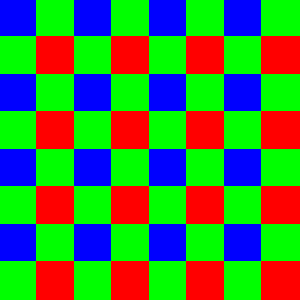
\includegraphics[scale=0.36]{imagenes/BayerFilter}
	\label{Bayer}
  \end{center}
\end{figure}


Ahora bien, esto genera una imagen que se aproxima a la realidad sólo en parte ya que para cada p\'ixel de la imagen tenemos la informaci\'on de s\'olo uno de sus tres canales. A causa de esto es que la misma debe ser reconstruida algorítmicamente, interpolando los valores de los colores que no fueron almacenados explícitamente para cada pixel.


En este punto adquieren relevancia las diferentes propuestas de reconstrucción de la imagen original. Esto conlleva la ejecución de diversos procedimientos, entre los que se encuentran el demosaicing, el análisis del balance de blancos, la curva tonal, la saturación y el contraste y la compresión final de la imagen. Como nuestra propuesta se aboca al primer paso mencionado, exploraremos en el presente trabajo sólo un subconjunto de una serie de variaciones no finita que admiten métodos de debayering como ser la interpolación por asignación de valores próximos, la interpolación bilineal y interpolación direccional.\\

A efectos de nuestro caso de estudio, la imagen bajo el Color Filter Array Bayer la vamos a generar sint\'eticamente, es decir mediante un algoritmo que tome una imagen original y devuelva una imagen de este formato. Esto nos permitir\'a hacer comparaciones entre los m\'etodos y la imagen original, teniendo as\'i un punto de referencia en cuanto a la correctitud de la imagen.

\newpage
\subsection{Inconvenientes de aproximar mediante el Polinomio de Lagrange}


Es nuestra intención exponer ahora el motivo que consideramos suficiente para decidir interpolar los valores ausentes a través de Splines en lugar de hacer uso del polinomio de Lagrange.\\
Sea dada la siguiente muestra: \\
\smallskip


\begin{tabular}{ | c || c | c | c | c | c |c | c | c | c | c | c | c | c | c | c |}
 \hline                 
   x & 1 & 2 & 3 & 4 & 5 & 6 & 7 & 8 & 9 & 10 & 11 & 12 & 13 & 14 \\
 \hline    
y & 10 & 10 & 10& 10& 10& 10& 10& 10& 10& 10& 10& 10& 10& 10 \\
 \hline  
 \end{tabular}

\smallskip

\begin{tabular}{  | c || c | c | c | c | c |c | c | c | c | c | c | c | c | c | c |}
 \hline                 
   x&15& 16 & 17 & 18 & 19 & 20 & 21 & 22 & 23 & 24 & 25 & 26 & 27 & 28\\
 \hline    
y & 10 & 10 & 10& 10& 10& 10& 10& 10& 10& 10& 10& 10& 10& 10 \\
 \hline  
 \end{tabular}
\bigskip
\\
El polinomio de Lagrange que interpola cada uno de esos valores tiene una expresión equivalente al Spline que lo hace, siendo su gráfico el que se muestra a continuación:
\smallskip

\begin{figure}[h!]
	\caption{}
	\begin{center}
	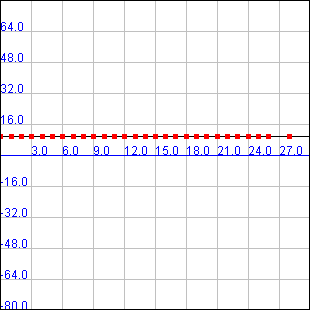
\includegraphics[scale=1]{imagenes/LagrangeSplinesCTE}
	\label{LagrangeSplinesCTE}
  \end{center}
\end{figure}

Supongamos ahora que el resultado de una medición - digamos $x_{12}$ - haya sido calculada con un ruido que represente el 1\% del valor real, modificándose la muestra de la siguiente forma:\\

\smallskip

\begin{tabular}{ | c || c | c | c | c | c |c | c | c | c | c | c | c | c | c | c |}
 \hline                 
   x & 1 & 2 & 3 & 4 & 5 & 6 & 7 & 8 & 9 & 10 & 11 & 12 & 13 & 14 \\
 \hline    
y & 10 & 10& 10& 10& 10& 10& 10& 10& 10& 10& 10& 10,1& 10 & 10\\
 \hline  
 \end{tabular}

 \smallskip

\begin{tabular}{  | c || c | c | c | c | c | c | c | c | c | c | c | c | c | c | }
 \hline                 
   x&15& 16 & 17 & 18 & 19 & 20 & 21 & 22 & 23 & 24 & 25 & 26 & 27 & 28\\
 \hline    
y & 10 & 10 & 10& 10& 10& 10& 10& 10& 10& 10& 10& 10& 10& 10 \\
 \hline  
 \end{tabular}

\bigskip

 En este caso se obtendría el gráfico representado en la Figura \ref{LagrangeX12a101} para el polinomio de Lagrange (escalado en la Figura \ref{LagrangeX12a101(zoomOut)})y el que se ilustra en la Figura \ref{SplinesX12a101} para el obtenido mediante Splines.\\

\begin{figure}[h!]
	\caption{}
	\begin{center}
	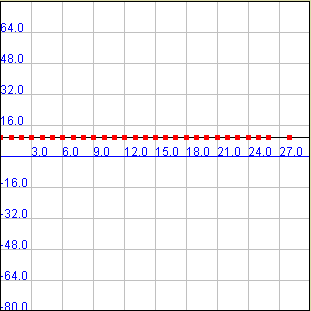
\includegraphics[scale=1]{imagenes/SplinesX12a101}
	\label{SplinesX12a101}
  \end{center}
\end{figure}

\begin{figure}
	\caption{}
	\begin{center}
	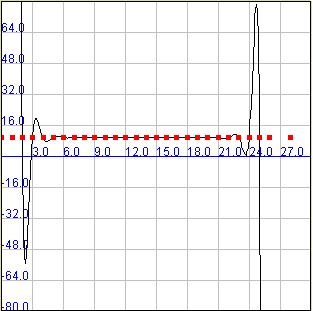
\includegraphics[scale=1]{imagenes/LagrangeX12a101}
	\label{LagrangeX12a101}
  \end{center}
\end{figure}

\begin{figure}
	\caption{}
	\begin{center}
	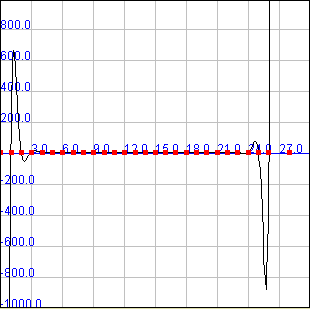
\includegraphics[scale=1]{imagenes/LagrangeX12a101(zoomOut)}
	\label{LagrangeX12a101(zoomOut)}
  \end{center}
\end{figure}

Como se puede observar, para la construcción del Spline el cambio en un valor de la imagen no impactó de una forma apreciable sobre el resto del polinomio. Sin embargo, el nuevo resultado generó un polinomio de Lagrange cuya diferencia con la Figura \ref{SplinesX12a101} es grosera en determinados intervalos.\\ 

Si se profundizara el error de la medición de acuerdo con la tabla presentada a continuación, notaríamos que el polinomio de Lagrange comenzaría a presentar una mayor cantidad de intervalos con valores drásticamente alejados de los dados como referencia. Por otro lado, Splines únicamente presentará variaciones en un entorno de los intervalos cuyos valores hayan sido modificados. Esto se puede  constatar en las Figuras \ref{SplinesX12a20}, \ref{LagrangeX12a20} y  \ref{LagrangeX12a20(zoomOut)}.\\


\begin{tabular}{ | c || c | c | c | c | c |c | c | c | c | c | c | c | c | c | c |}
 \hline                 
   x & 1 & 2 & 3 & 4 & 5 & 6 & 7 & 8 & 9 & 10 & 11 & 12 & 13 & 14 \\
 \hline    
y & 10 & 10& 10& 20& 10& 10& 10& 10& 10& 10& 10& 20& 10 & 10\\
 \hline  
 \end{tabular}

\smallskip

\begin{tabular}{  | c || c | c | c | c | c | c | c | c | c | c | c | c | c | c | }
 \hline                 
   x&15& 16 & 17 & 18 & 19 & 20 & 21 & 22 & 23 & 24 & 25 & 26 & 27 & 28\\
 \hline    
y & 10 & 10 & 10& 10& 10& 10& 10& 10& 10& 10& 10& 10& 10& 10 \\
 \hline  
 \end{tabular}

\begin{figure}
	\caption{}
	\begin{center}
	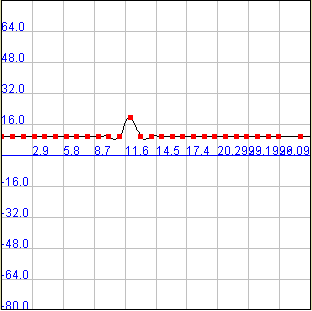
\includegraphics[scale=1]{imagenes/SplinesX12a20}
	\label{SplinesX12a20}
  \end{center}
\end{figure}

\begin{figure}
	\caption{}
	\begin{center}
	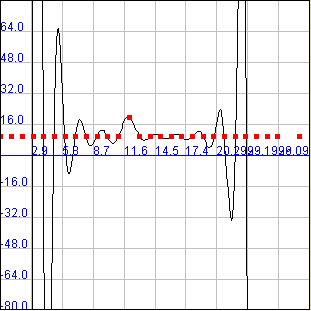
\includegraphics[scale=1]{imagenes/LagrangeX12a20}
	\label{LagrangeX12a20}
  \end{center}
\end{figure}

\begin{figure}
	\caption{$Zoom \ out$ de la Figura \ref{LagrangeX12a20}}
	\begin{center}
	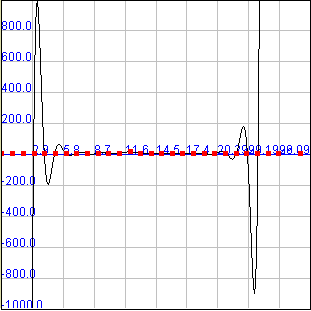
\includegraphics[scale=1]{imagenes/LagrangeX12a20(zoomOut)}
	\label{LagrangeX12a20(zoomOut)}
  \end{center}
\end{figure}

\bigskip

\newpage
En conclusión, el polinomio de Lagrange se comporta de una manera menos predecible estable entre dos variables independientes y no garantiza que en esos intervalos el valor de la función sea cercano a los ya conocidos.\\
La carencia de predictibilidad hace del polinomio de Lagrange una mala alternativa para la interpolación, en comparación con las ventajas proporcionadas por el empleo de Splines.\\




\newpage
\subsection{M\'etricas de comparaci\'on de im\'agenes}

Con el fin de establecer una relaci\'on entre las im\'agenes obtenidas con los distintos m\'etodos y la imagen original es que nace la necesidad de contar con \emph{M\'etricas de comparaci\'on de im\'agenes}.\\

Existen dos m\'etodos dentro de los mecanismos usados:

\emph{Subjetivos:} Son los conceptos que una persona puede detectar visualmente.

\emph{Objetivos:} Son operaciones matem\'aticas en el dominio bidimensional o tridimensional de im\'agenes orientados a determinar la variaci\'on presente en una imagen.\\

Las métricas subjetivas u objetivas se pueden usar con comparación respecto a una referencia o sin considerarla.\\

En nuestro caso de estudio, nos vamos a centrar en la comparaci\'on de la imagen original y la obtenida a trav\'es de los distintos m\'etodos. Por esto mismo, vamos a usar m\'etricas que cuenten con una imagen de referencia.\\

 Dos de las m\'etricas m\'as sencillas son el \emph{\textbf{Error cuadr\'atico Medio}} (mse) y \emph{\textbf{Peak signal-to-noise ratio}} (psnr). Ambas cuentan con la capacidad de an\'alisis p\'ixel por p\'ixel.\\

\[
 \textbf{mse} = \frac{1}{mn} \sum_{i=0}^{m-1} \sum_{j=0}^{n-1} [I(x,y) - K(x,y)]^2
\]
  \indent \indent \indent \textit{Donde I y K son imágenes a comparar de tamaño $mxn$.}



\[
 \textbf{psnr} = 10 \log \frac{(2^n-1)^2}{mse} = 10 \log \frac{255^2}{mse}
\]

Otro tipo de medidas a tener en cuenta son las que utilizan indicadores de la imagen similares a los presentes en la visi\'on humana, como es el caso de \emph{\textbf{Structural similarity}} (ssim) que es una funci\'on que depende de la luminiscencia, el contraste y la similaridad estructural.

\[
 \textbf{ssim}(x,y) = \frac{(2\mu_x\mu_y+c_1)(2\sigma_{xy}+c_2)}{(\mu_x^2+\mu_y^2+c_1)(\sigma_x^2+\sigma_y^2+c_2)}
\]

\noindent Donde, 

$\mu_x$ es la esperanza de $x$

$\mu_y$ es la esperanza de $y$

$\sigma_x^2$ es la varianza de $x$

$\sigma_y^2$ es la varianza de $y$

$\sigma_{xy}$ es la covarianza entre $x$ e $y$

$c_1 = (k_1L)^2$ ; $c_2 = (k_2L)^2$ son dos variables que estabilizan la divisi\'on con un denominador chico

$L$ es el rango din\'amico de los valores de los p\'ixeles (com\'unmente es $2^{\#bitsPorPixel}-1$)

$k_1 = 0,01$ y $k_2 = 0,03$ por default\\

Las m\'etricas que vamos a utilizar nosotros como m\'etodo de comparacion de im\'agenes son \emph{psnr} y \emph{ssim}. Los cuales calcularemos con sus instrucciones respectivas en Matlab$\textregistered$.

\newpage
\subsection{Artifacts}
\textcolor{red}{Explicar cada artifact y agregar grid}

Como se explicó anteriormente, dos de los tres canales de cada p\'ixel son interpolados algorítmicamente. Si bien los métodos que pueden proponerse a tal fin no son limitados, un subconjunto de ellos producirá imágenes que diferirán considerablemente de las que quisieron ser capturadas originalmente. 

Para evaluar el peso de estas diferencias  existen mecanismos cuantitativos (como los mencionados en el apartado \emph{M\'etricas de comparaci\'on de im\'agenes}) y otros de tipo cualitativo. Un grupo de estos últimos está constituido por la exploración de \textit{artifacts}.

Los \textit{artifacts} son efectos visuales indeseados frecuentes que se producen sobre la imagen procesada a causa de una interpolación poco conveniente. 

Ejemplos de artifacts son el efecto <<\emph{Blurring}>>(Figura \ref{blurring}), el <<\emph{False color}>>(Figura \ref{false}), el <<\emph{Jaggies}>>(Figura \ref{jaggies}),   el <<\emph{efecto Moiré}>>(Figura \ref{moire}) y el <<\emph{Zipper}>>(Figura \ref{zipper}).


\begin{figure}[h!]
	\caption{A la izquierda, la imagen original. A la derecha, la que presenta <<blurring>>.}
	\begin{center}
	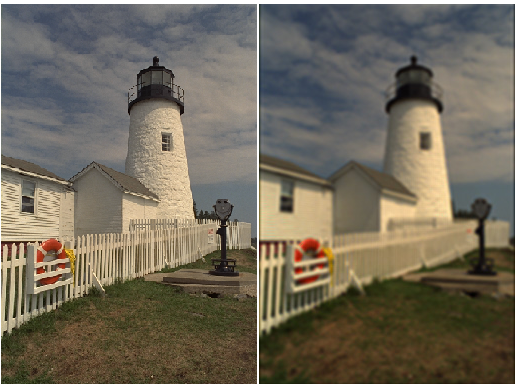
\includegraphics[scale=0.66]{imagenes/blurring}
	\label{blurring}
  \end{center}
\end{figure}

\begin{figure}[h!]
	\caption{A la izquierda, la imagen original. A la derecha, la que presenta <<false color>>.}
	\begin{center}
	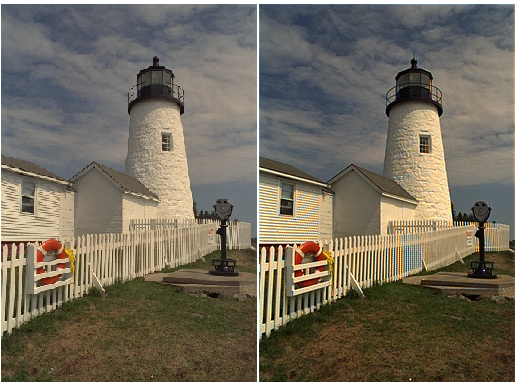
\includegraphics[scale=0.66]{imagenes/false}
	\label{false}
  \end{center}
\end{figure}

\newpage

\begin{figure}[h!]
	\caption{A la izquierda, la imagen original. A la derecha, la que presenta <<zipper>>.}
	\begin{center}
	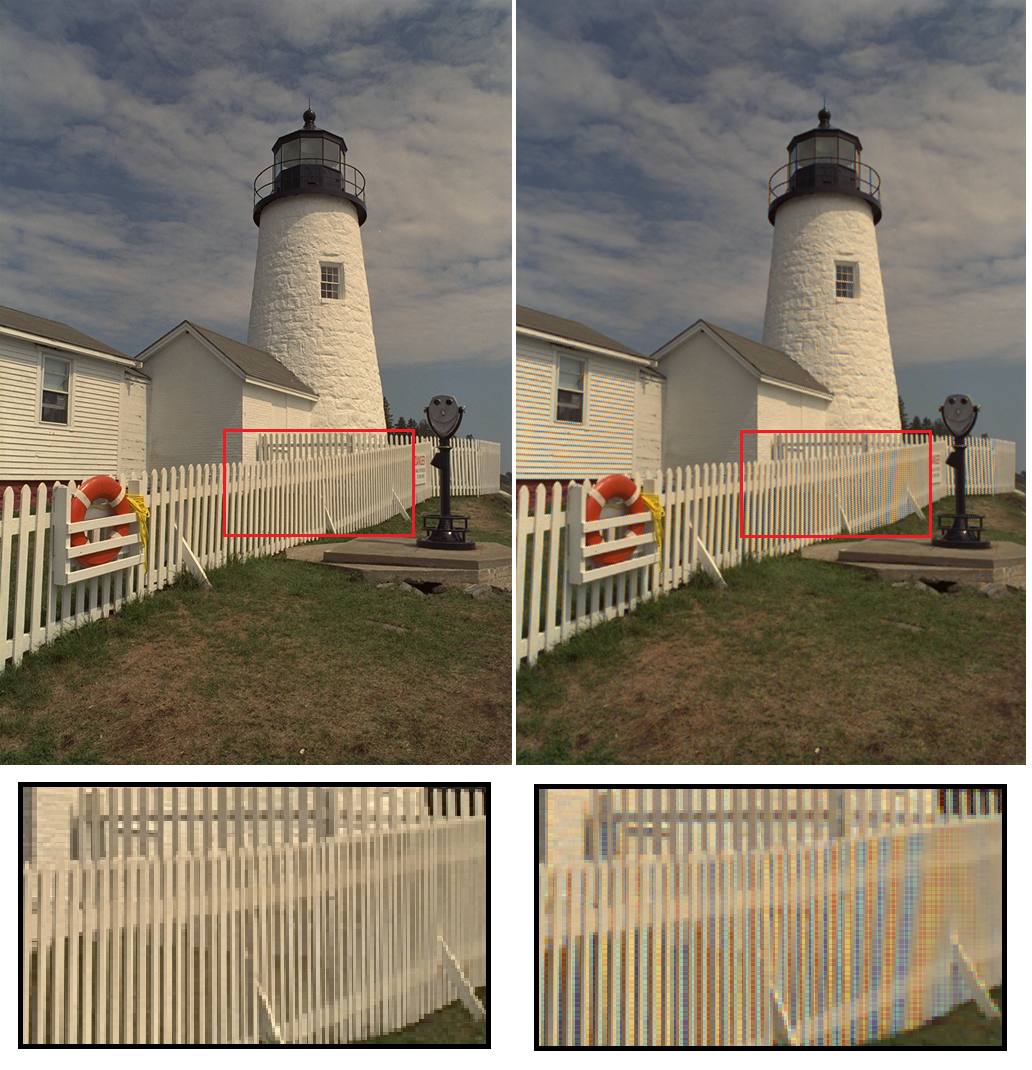
\includegraphics[scale=0.50]{imagenes/zipper}
	\label{zipper}
  \end{center}
\end{figure}

\begin{figure}[h!]
	\caption{A la izquierda, la imagen original. A la derecha, la que presenta <<jaggies>>.}
	\begin{center}
	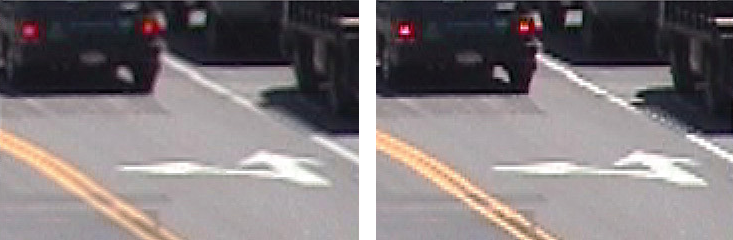
\includegraphics[scale=0.50]{imagenes/jaggies}
	\label{jaggies}
  \end{center}
\end{figure}

\newpage

\begin{figure}[h!]
	\caption{A la izquierda, la imagen original. A la derecha, la que presenta el efecto <<moiré>>.}
	\begin{center}
	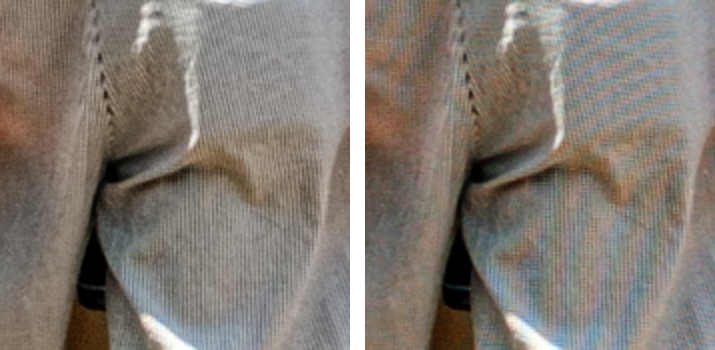
\includegraphics[scale=0.50]{imagenes/moire}
	\label{moire}
  \end{center}
\end{figure}







\textcolor{red}{ESTARÍA BUENO AGREGAR TIPO ANECDÓTICO LOS ARTIFACTS DEL OJO HUMANO (?) PERO NO SÉ EN PRINCIPIO CÓMO MECHARLO ACÁ}





\newpage
\section{Desarrollo}

Dada una \textit{imagen cruda}, los valores que contiene en sus píxeles para cada canal los asumimos reales y ciertos. Por lo tanto, resta averiguar para cada uno de ellos los valores de los dos canales para los cuales dicha información se encuentra ausente.

\subsection{Vecino m\'as cercano}
La implementación más sencilla para la estimación de los canales desconocidos de cada pixel consiste en otorgar a cada canal ``vacío'' el valor real m\'as pr\'oximo que corresponda a dicho color. Este m\'etodo es algor\'itmicamente asequible, pero no tiene en cuenta dos factores: \\
\\

$\triangleright$ Por un lado, al otorgar el valor de un sólo pixel cercano, surge la necesidad de definir arbitrariamente cuál se debe escoger como valor referencial en casos en que un conjunto de pixeles son equidistantes al analizado y no existe un criterio claro acerca de cuál de ellos debe ser considerado el ``más próximo''. Que esta decisión impacte en el resultado de forma inocua o parcial o totalmente nociva dependerá en cierta medida de la fotografía que se esté analizando.

El ejemplo más trivial se encuentra en una imagen monocromática: al ser los valores reales idénticos para todos los pixeles, tomar las magnitudes de cualquier otra posición para cada canal correspondiente no afectará el resultado final. Sin embargo, si consideráramos una imagen formada por columnas alternadas de un pixel de ancho rojas (\#0000FF) y blancas (\#FFFFFF), entonces si para definir los canales verde y azul de un pixel rojo se tomara como posiciones más cercanas aquel que se encuentra debajo suyo y el que está a la derecha del mismo (respectivamente), el resultado sería un pixel fucsia (\#FF00FF). En cambio, si los pixeles elegidos fueran su inmediato derecho y en el que se encuentra a su diagonal inferior derecha, la posición analizada debería manifestar el color blanco (\#000000).

Si bien se trata de un ejemplo de alcance limitado, resulta suficiente para ilustrar los potenciales problemas de la aplicación de este algoritmo.\\

\textcolor{red}{Aca va la fotito que tiene que armar Belu}\\

$\triangleright$ Por otra parte - y en cierta forma vinculado al ejemplo anterior - este método no especifica ninguna distinción respecto de la forma de proceder en casos de borde o de superficies parejas. \\


\newpage
\subsection*{Decisiones tomadas en el Algoritmo de Vecino M\'as Cercano}

A la hora de formular nuestro algoritmo de Vecino m\'as Cercano nos vimos obligados a determinar aspectos que conciernen al dise\~no del mismo. 

La principal decisi\'on que debimos tomar fue con qu\'e criterio elegir al p\'ixel m\'as cercano cuando no es \'unico (esto ocurre en todos los casos). 

\begin{figure}[h!]
	\caption{}
	\begin{center}
	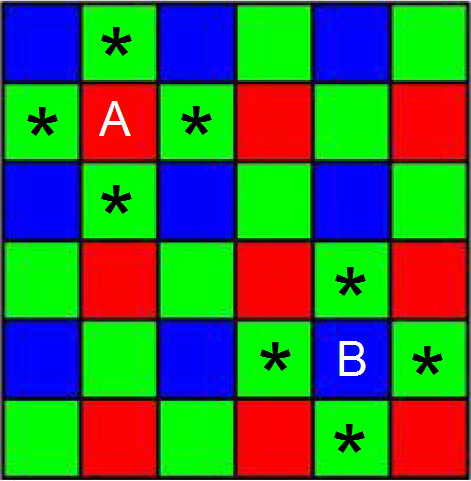
\includegraphics[scale=0.36]{imagenes/vecino1}
	\label{Vecino1}
  \end{center}
\end{figure}

Para determinar el valor del canal verde sobre un p\'ixel definido rojo\emph{(A)} o azul\emph{(B)} tenemos cuatro p\'ixeles a la misma distancia (1) que nos brindan informaci\'on sobre el canal verde. 
\begin{figure}[h!]
	\caption{}
	\begin{center}
	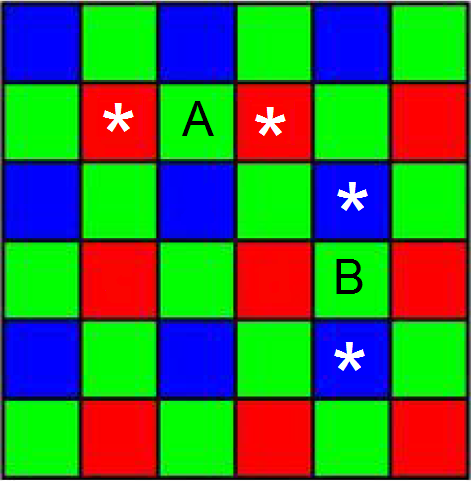
\includegraphics[scale=0.36]{imagenes/vecino2}
	\label{Vecino2}
  \end{center}
\end{figure}

Si nos situamos en un p\'ixel naturalmente verde, tanto para determinar su canal rojo\emph{(A)} como para determinar su canal azul\emph{(B)} sus p\'ixeles m\'as cercanos que nos brindan informaci\'on son dos (a 1 de distancia cada uno). 
\begin{figure}[h!]
	\caption{}
	\begin{center}
	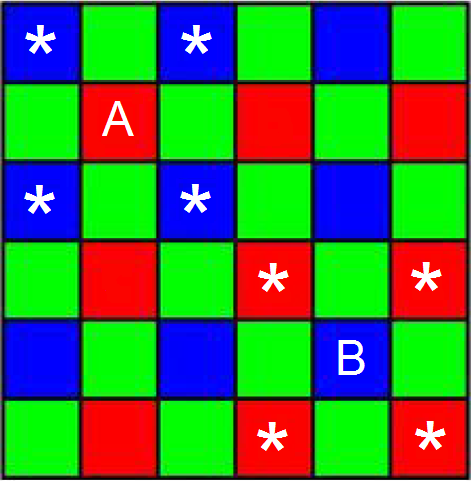
\includegraphics[scale=0.36]{imagenes/vecino3}
	\label{Vecino3}
  \end{center}
\end{figure}

Y por \'ultimo para determinar el valor del canal azul sobre un p\'ixel de origen rojo\emph{(A)} (y viceversa\emph{(B)}) nos encontramos con cuatro p\'ixeles a la misma m\'inima distancia (2) en sus diagonales. \\

Por este motivo, realizamos dos versiones de este algoritmo variando en ellas cu\'al p\'ixel elegir para rellenar el canal verde cuando se est\'a situado sobre un p\'ixel azul o rojo.

En el \emph{\textbf{algoritmo 1}} si se est\'a en un p\'ixel rojo se elige al de arriba y si se est\'a en un p\'ixel azul se elige el de la derecha. En cambio, en el \emph{\textbf{algoritmo 2}} si se est\'a en un p\'ixel rojo se elige al de la izquierda y si se est\'a en un p\'ixel azul se elige al de abajo.

Corrimos ambos algoritmos con diversas fotos, a continuaci\'on se muestran algunos ejemplos que contienen detallado el valor de psnr y ssim para cada imagen respecto de la original.

\begin{figure}[h!]
	\caption{}
	\begin{center}
	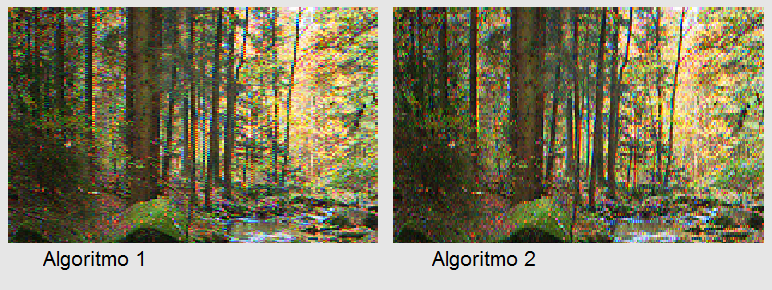
\includegraphics[scale=0.60]{imagenes/Vecino/arbolitos}
	\label{arbolitos}
	
	psnr1 =   14.3119

psnr2 =   14.3533

ssim1 =    0.3819

ssim2 =    0.3856
  \end{center}
\end{figure}

\begin{figure}[h!]
	\caption{}
	\begin{center}
	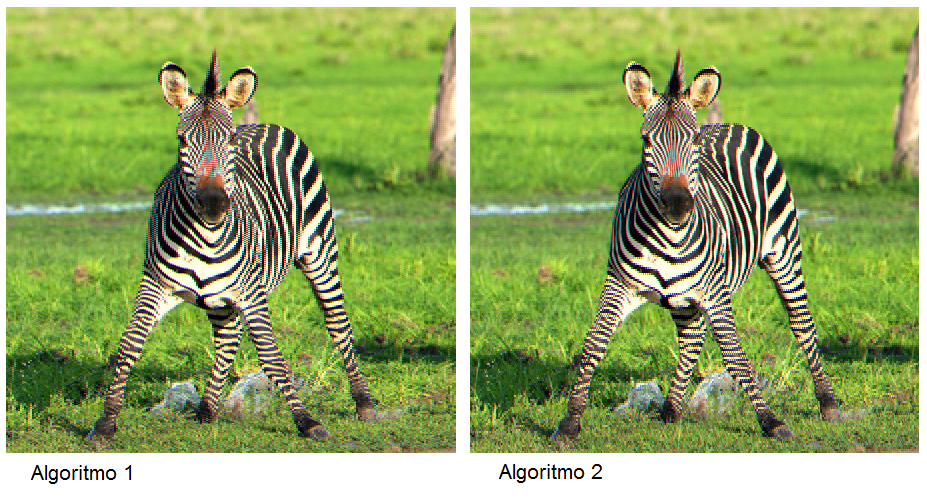
\includegraphics[scale=0.60]{imagenes/Vecino/zebraCara}
	\label{zebraCara}
	
	psnr1 =   19.8295

psnr2 =   20.0706

ssim1 =    0.8806

ssim2 =    0.8841
  \end{center}
\end{figure}

\newpage
\begin{figure}[h!]
	\caption{}
	\begin{center}
	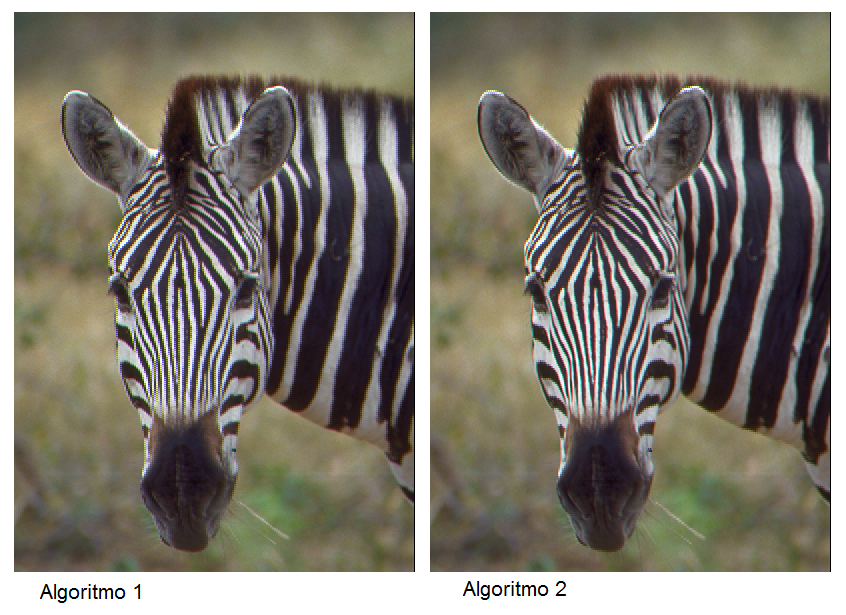
\includegraphics[scale=0.60]{imagenes/Vecino/zebra}
	\label{Zebra}
	
	psnr1 =   21.1167

psnr2 =   21.3368

ssim1 =    0.8374

ssim2 =    0.8417
  \end{center}
\end{figure}


\begin{figure}[h!]
	\caption{}
	\begin{center}
	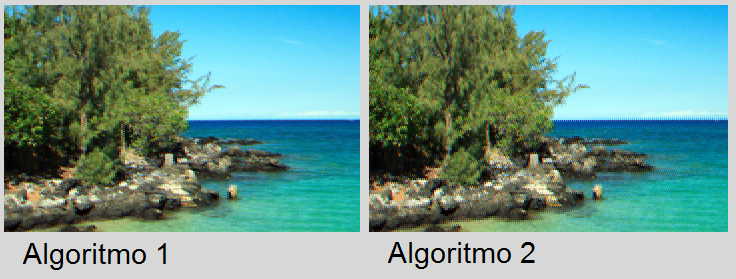
\includegraphics[scale=0.06]{imagenes/Vecino/hawaiicmp}
	\label{Zebra}
	
	psnr1 =   23.2721

psnr2 =   23.2371

ssim1 =    0.8560

ssim2 =    0.8553
  \end{center}
\end{figure}

\newpage

\begin{figure}[h!]
	\caption{}
	\begin{center}
	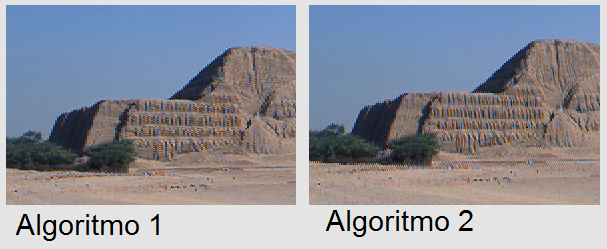
\includegraphics[scale=0.06]{imagenes/Vecino/piramides3cmp}
	\label{Zebra}
	
	psnr1 =   23.8518

psnr2 =   23.8270

ssim1 =    0.7514

ssim2 =    0.7515
  \end{center}
\end{figure}

\begin{figure}[h!]
	\caption{}
	\begin{center}
	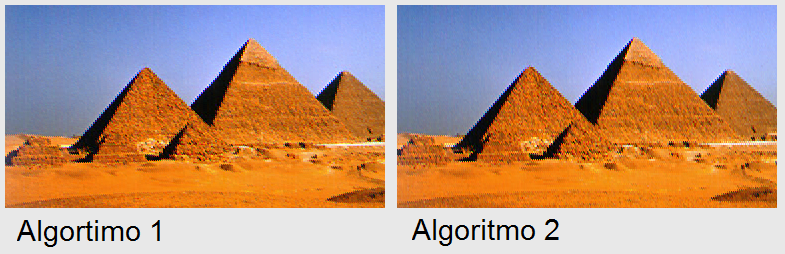
\includegraphics[scale=0.70]{imagenes/Vecino/piramides2cmp}
	\label{Zebra}
	
	psnr1 =   21.7691

psnr2 =   21.7494

ssim1 =    0.9508

ssim2 =    0.9506
  \end{center}
\end{figure}




Se puede apreciar que el Algoritmo 1 es capaz de delimitar mejor bordes que poseen rayas en forma horizontal, en cambio el Algoritmo 2 le da una mejor definici\'on a los bordes verticales. Dada la forma de la implementaci\'on, las anomal\'ias observadas en las imagenes cobran sentido.\\


Debido a que no se puede establecer con un criterio cu\'al es m\'as correcta que la otra, ya que la veracidad de la imagen obtenida var\'ia depende la imagen inicial y su estructura. Nosotros optamos por utilizar el \emph{\textbf{Algoritmo 1}}.\\

\textit{Se adjuntan las im\'agenes en su tama\~no original.}

\newpage
\subsection{Interpolaci\'on Bilineal}

La interpolación bilineal es una composición de interpolaciones lineales en dos direcciones diferentes. Este método desmerece el caracter arbitrario de asignación de un canal a partir del valor más próximo para el mismo y propone que el resultado final sea calculado teniendo en cuenta y promediando todos los valores cercanos sin priorizar ninguno de ellos. \\

Como la estructura del filtro Bayer sólo asegura para los p\'ixels nativamente azules o rojos tener todas sus posiciones vecinas netamente verdes, aquel es el único caso en que el cálculo de un canal se reduce a computar el promedio de los valores superior, inferior, derecho e izquierdo al espacio que se quiere interpolar.\\

Sin embargo, si se quisiera obtener el valor de azul o rojo que correspondería asignar a un p\'ixel nativamente verde, el entramado de Bayer obligaría a estimarlo a partir de sus dos valores m\'as cercanos ubicados a la derecha e izquierda o arriba y abajo dependiendo de la ubicaci\'on del p\'ixel. \\

Por otro lado, los valores del canal azul para un p\'ixel rojo (y los del canal rojo para un p\'ixel azul) se calcularían tomando en cuenta las cuatro posiciones diagonales a la analizada. Este proceso no se realizar\'ia simplemente tomando el promedio de sus cuatro diagonales sino que requeriría tomar dos p\'ixels cercanos que pertenezcan a la misma fila o columna, cuyo canal real sea el verde, calcular sus valores de azul/rojo promediando los de las casillas nativas azules/rojas más próximas y posteriormente realizar un nuevo promedio entre los valores resultantes.\\

Tomando como referencia la ilustración \ref{bilineal} se puede ver que el cálculo recien descripto equivale a calcular el valor en el canal rojo para el p\'ixel x. Lo cual consistir\'ia en: 

\begin{itemize}
 
\item Hacer el promedio entre \textit{a y b} y luego, ubicar ese valor para el canal rojo para el p\'ixel ubicado arriba de x.

\item Hacer el promedio entre \textit{c y d} y luego, ubicar ese valor para el canal rojo para el p\'ixel ubicado debajo de x.

\item Una vez obtenidos estos dos valores, promediarlos y ubicarlos en el canal rojo de x.\\
\end{itemize}
Llegando as\'i a que realizar este c\'alculo es equivalente a realizar el promedio entre los valores de sus diagonales:

\[
 \frac{\frac{a+b}{2} + \frac{c+d}{2}}{2} = \frac{a+b+c+d}{4}
\]

\begin{figure}[h!]
	\caption{}
	\begin{center}
	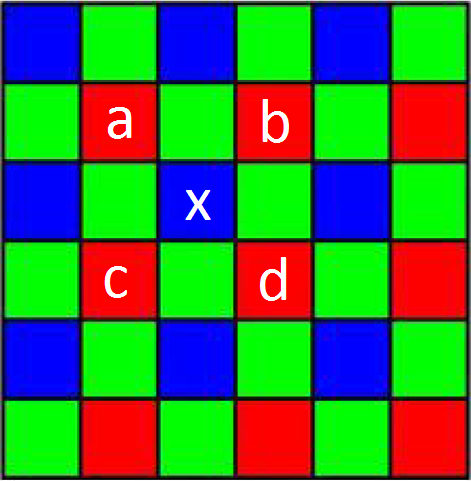
\includegraphics[scale=0.36]{imagenes/bilineal}
	\label{bilineal}
  \end{center}
\end{figure}

\newpage
\subsection{Interpolaciones Direccionales}
Se trata de una gran cantidad de métodos que buscan comenzar a resolver el problema de demosaicing realizando inicialmente una interpolación en una dirección y combinando con algún criterio determinado el resultado estimado con el obtenido de una aproximación realizada en otra dirección.\\

La implementación de este tipo de métodos exige tomar al menos dos decisiones de peso que distinguirán a unos de otros:\\

\begin{itemize}
    \item De qué forma se realizarán las interpolaciones (en qué direcciones y mediante qué mecanismo de interpolación)
    \item Con qué criterio y consideraciones combinar la información proporcionada por las direcciones escogidas.
\end{itemize}

Para escoger alguna opción apropiada corresponde analizar las características del Color Filter Array con el que se va a trabajar, puesto que no todas las direcciones van a aportar en la totalidad de los casos la misma información.

En cuanto a la combinación de los resultados de las distintas interpolaciones, es conveniente tener presente que el promedio de los mismos no es siempre una buena opción. Por ejemplo, supongamos que se analiza una imagen que presenta en un sector las características observables en la Imagen original de la ilustración \ref{apxl1}.


\begin{figure}[h!]
	\caption{}
	\begin{center}
	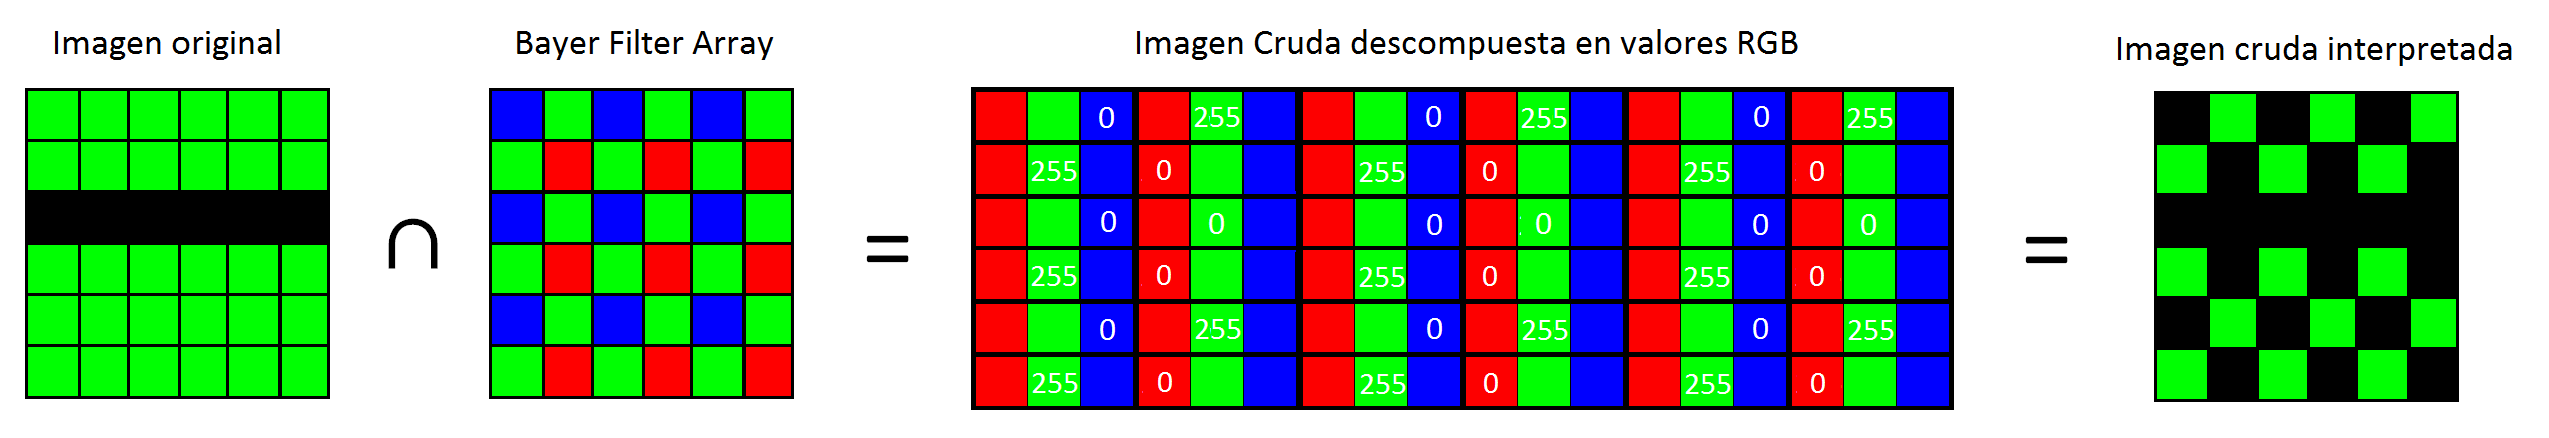
\includegraphics[scale=0.23]{imagenes/apxl1}
	\label{apxl1}
  \end{center}
\end{figure}

En dicha figura se analiza la información de la misma que sería captada por los fotosensores respondiendo al Bayer Filter Array. 

En el esquema \ref{apxl2} se puede observar que para varios p\'ixeles la interpolación horizontal retorna valores distintos a la realizada verticalmente (esto tiene sentido, pues se trata de un área homogénea atravesada por una fila de distinto color).

El resultado de empleo del promedio como estrategia de nivelacion de dichos valores queda expuesto en la Figura \ref{apxl3}, en la cual se puede observar el causante del artifact ``zipping'', producto de un algoritmo indiferente ante los cambios de color abruptos.\\

\begin{figure}[h!]
	\caption{}
	\begin{center}
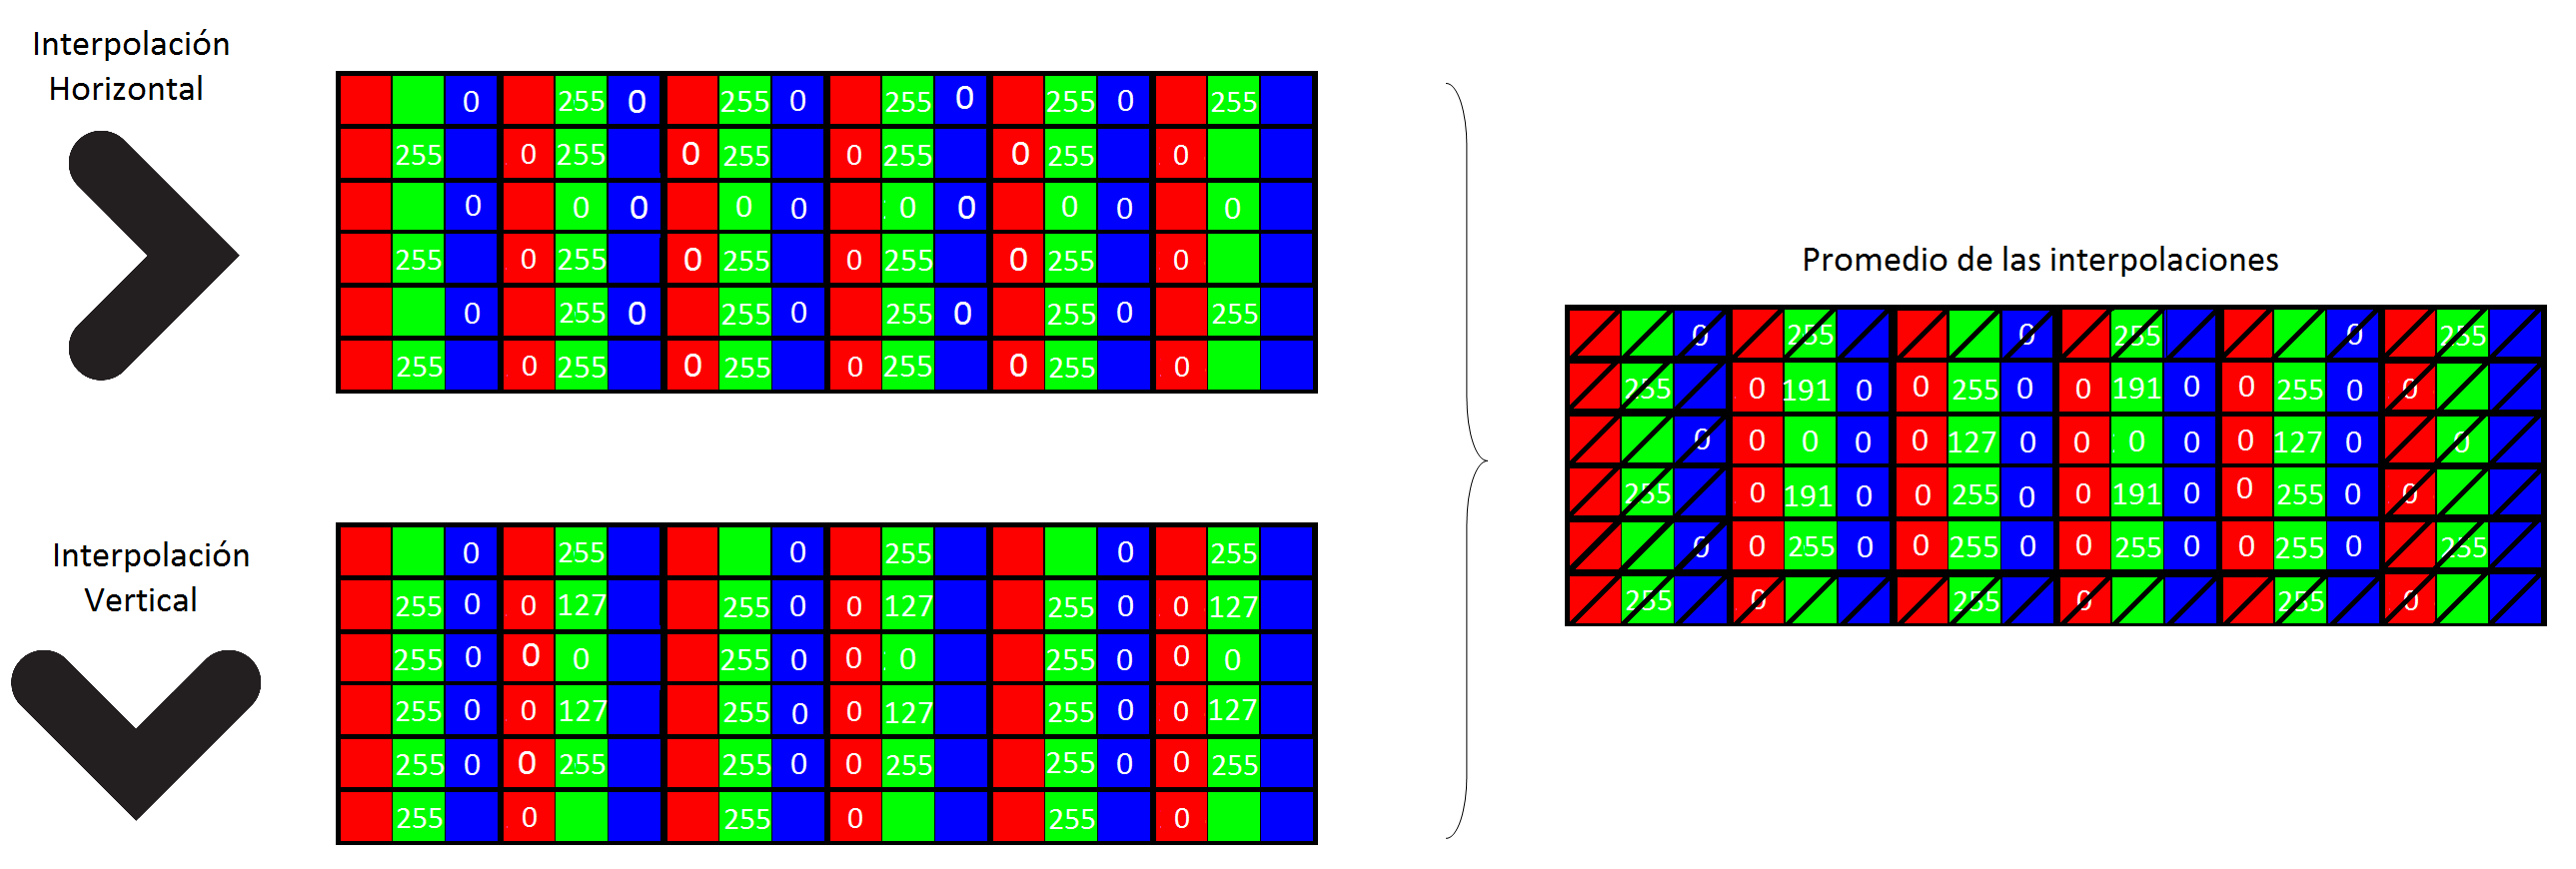
\includegraphics[scale=0.26]{imagenes/apxl2}
	\label{apxl2}
  \end{center}
\end{figure}

\begin{figure}[h!]
	\caption{}
	\begin{center}
	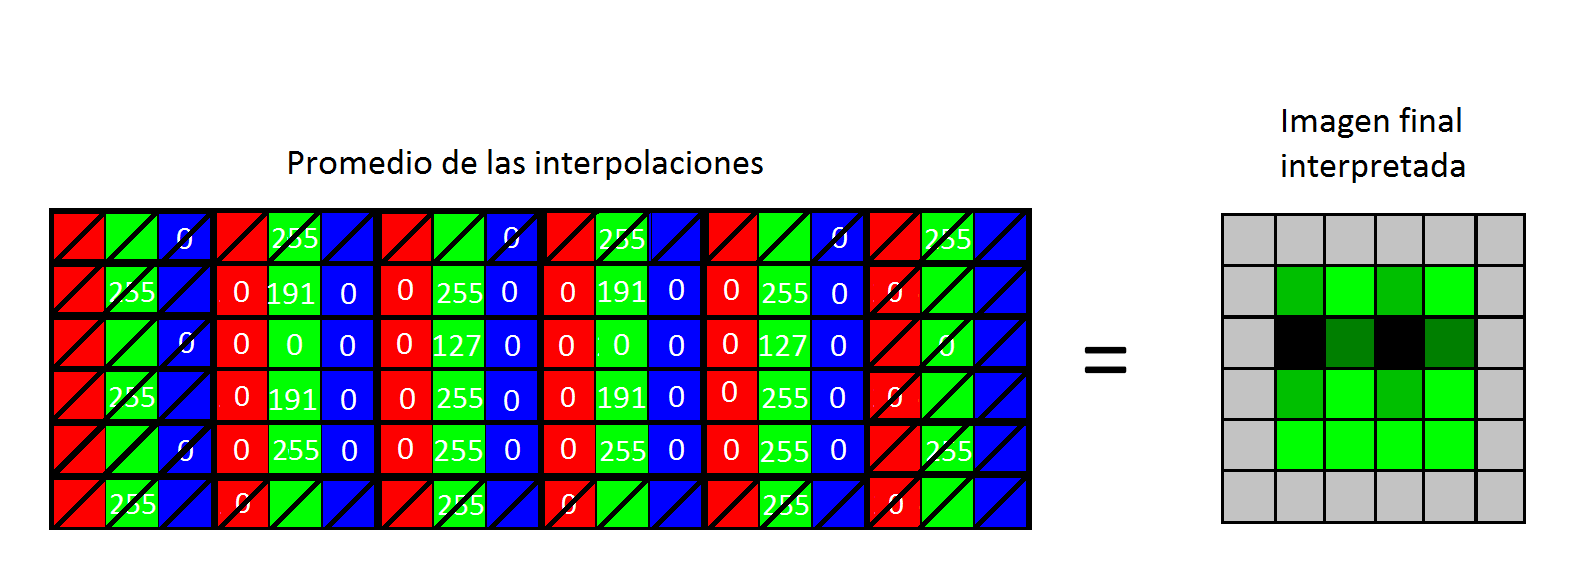
\includegraphics[scale=0.36]{imagenes/apxl3}
	\label{apxl3}
  \end{center}
\end{figure}

\newpage
Ciertamente esto no es lo esperado y existen mecanismos que permiten corregir este error. Uno de ellos consiste en calcular el gradiente del color para utilizarlo al combinar los resultados, de modo tal que si el mismo fuera de gran magnitud (es decir, la variación del color es considerable) entonces el peso que debe tener el valor calculado en el resultado final debería ser menor a aquel que fue calculado en una dirección cuyo gradiente fuera menor (es decir, que se tratara de una superficie más cromáticamente homogénea).



\pagebreak

\newpage
\subsection{Splines}
\subsubsection*{Generación de los Splines}
\textcolor{red}{No se si estan de acuerdo, pero no me pareceria mal dividir un poco la intro teórica en este TP, y hablar acá de por qué no usamos Lagrange. Si no les parece da igual, acá se puede hacer referencia a eso. Y listo (es lo que voy a dejar escrito ahora) pero hay que meditar qué queda mejor.}

\textcolor{blue}{Hablar de todos sus tipos\\
Decir que bilineal y poner 0.5 queda igual (o casi igual je), usar psnr.\\
Y ver cual vamos a dejar\\
Y que usamos NATURALES}

Yendo un paso más allá de la interpolación bilineal, podemos preguntarnos qué otros métodos existen que nos permitan obtener mejores resultados. Una buena primera idea sería analizar qué sucede con los Splines. \\

Los Splines (o trazadores cúbicos) son un tipo particular de interpoladores fragmentarios: funciones partidas que interpolan a través de polinomios un conjunto de puntos. En el caso de los Splines, se interpola entre dos puntos mediante un polinomio cúbico.\\

Como fue explicado anteriormente, los Splines son una opción muy buena a la hora de interpolar funciones: en el análisis realizado contra el Polinomio de Lagrange pudimos observar que este último puede llegar a ser excesívamente malo en ciertos casos. Considerando la superioridad de los Splines, entonces, nos propusimos encontrar un algoritmo que los utilice para conseguir buenas interpolaciones que generen imagenes de calidad superior a la hora de realizar el demosaicing.\\

Conseguir el Spline interpolador dado un conjunto de $N$ puntos $X_j$ consiste en resolver un sistema tridiagonal de $NxN$(\textcolor{red}{ACA PONER ALGUNA CITA DEL BURDEN O ALGO DE DONDE SACAR TODO EL TEMA DEL ARMADO DEL SISTEMA DEL SPLINE. No creo que sea correcto copiar acá la teorica entera sobre el tema (que encima fue eterna)}) que posea el siguiente aspecto (si trabajamos con splines naturales): \\

\textcolor{red}{Aca poner matriz, no se como se hace\\}

\noindent Donde $h_j$ es igual a la distancia entre los puntos $X_j$ y $X_{j+1}$. \\

Para nuestro problema en particular, vamos a considerar las funciones a interpolar como el valor de un canal de RGB en alguna porción de la imagen. Dada la fisonomía del Bayer Filter Array, puede observarse con facilidad que, tomando una fila o una columna cualesquiera, la distancia que hay entre dos píxeles del mismo color es de 2 unidades (es decir, para un p\'ixel azul en la posición $j$ de una fila, el siguiente p\'ixel azul se va a encontrar en la posición $j+2$). Esto incluso aplica a si tomamos diagonales (no las que contienen exclusivamente verde, aunque dicho caso no nos es de interés ya que no se interpolaría el verde sobre la misma). \\
Por esta razón, podemos reemplazar $h_j$ por 2, para todo $j$, y obtener la siguiente matriz: \\

\textcolor{red}{La otra matriz con 2-8-2\\}

Este sistema tiene la particularidad de ser estrictamente diagonal dominante, y por lo tanto va a tener solución única, con lo cual sabemos que el método interpolador funcionará correctamente. \\


\textcolor{red}{Poner los pseudocodigos y explicar brevemente la implementación (que se usó matriz esparsa, bla)\\}


\subsubsection*{Aplicación de Splines al problema de Demosaicing}

Una vez resuelto el problema de la implementación de los algoritmos que generan el spline e interpolan valores en el mismo, el siguiente paso fue pensar c\'omo aplicarlo al problema que nos concierne: el Demosaicing de imágenes. Diversos métodos fueron considerados y estudiados, y a continuación presentaremos los que creemos que son más representativos de la experimentación que realizamos. \\

El primer acercamiento que tuvimos con Splines fue simple: para cada p\'ixel, interpolar su fila y su columna por completo para los canales faltantes, y asignar el promedio entre ambos valores obtenidos. \\
A primera vista, este método aparenta ser muy parecido a la interpolación bilineal, razón por la cual decidimos comparar cualitativamente los outputs de ambos algoritmos:
\begin{itemize}
\item Subjetivamente, las imágenes son prácticamente idénticas para ambos métodos. Las diferencias son demasiado mínimas como para ser realmente apreciadas.
\item Objetivamente, mediciones de PSNR para distintas imágenes arrojaron valores sorpresivamente distintos (alrededor de 1 punto de diferencia), favoreciendo a la interpolación bilineal. \textcolor{red}{VER DE PONER MEDICIONES DE SSIM. No se si poner imagenes aca o en exploracion de artifacts?}
\end{itemize}

También fueron medidos los tiempos de ejecución para ambos algoritmos:\\

\textcolor{red}{tabla de tiempos?\\}

En vista de estos resultados, decidimos descartar (o mejor dicho, intentar mejorar) el algoritmo mediante Splines, ya que ni en tiempo ni en calidad lo encontramos superior.\\

El primer aspecto con el que decidimos experimentar fue la manera de combinar la información obtenida a través de las interpolaciones. En el caso anterior, simplemente realizábamos el promedio de los valores obtenidos al interpolar una fila y una columna. Sin embargo, este acercamiento no es siempre bueno, ya que puede traer resultados no deseados en los bordes. Es por esta razón que decidimos proponer una idea más sofisticada, detallada brevemente en la sección de interpolación bilineal: el uso del gradiente. \\

A modo de ejemplo, la derivada horizontal en el canal verde del p\'ixel puede estimarse de la siguiente manera:

\[|\partial_xG(x,y)| \approx |G(x-1,y) - G(x+1,y)|\]

Y, análogamente, la vertical:

\[|\partial_yG(x,y)| \approx |G(x,y-1) - G(x,y+1)|\]

Utilizando este concepto, modificamos nuestro algoritmo para que, en lugar de combinar la información obtenida mediante el promedio, haga lo siguiente:
\textcolor{red}{(ver de poner pseudocodigo aca en lugar de esto)}
\begin{itemize}
\item Interpolar por filas 
\item Al realizar la interpolación por columnas, para los p\'ixeles rojos y azules tenemos ahora dos valores posibles de verde. Comparamos los valores de las derivadas horizonal y vertical para el color verde:
\begin{itemize}
\item Si la derivada horizontal es mayor que la vertical, entonces le asignamos el valor de verde dado por la interpolación de la columna
\item Si la derivada vertical es mayor que la horizontal, entonces le asignamos el valor de verde dado por la interpolación de la fila
\end{itemize}
\end{itemize}

Aplicando este método, pudimos observar mejoras en varios de los bordes de nuestras imágenes: los mismos ahora son más suaves, y en algunos casos se disminuyó la visibilidad de los artifacts.\\

\textcolor{red}{poner fotitos}

A pesar de haber 


\newpage
\subsection{Algoritmo de Malvar, He y Cutler}

Luego de la lectura y estudio de la publicaci\'on \textit{HIGH-QUALITY LINEAR INTERPOLATION
FOR DEMOSAICING OF BAYER-PATTERNED COLOR IMAGES} \textbf{[2]}, nos decidimos por experimentar con el algoritmo planteado y as\'i observar las mejoras planteadas en este trabajo.\\

Malvar, He y Cutler presentan una cr\'itica a los m\'etodos que no utilizan los tres canales RGB en su conjunto, como por ej. la \emph{interpolaci\'on Bilineal} a la cual le adjudica la generaci\'on de significantes \textit{artifacts}. Y presentan un m\'etodo de Demosaicing en el cual el estudio de cada canal no se hace de manera independiente a los otros dos, que mejora en aspectos de tiempo de c\'omputo a algoritmos similares.\\

Los tres canales en su conjunto contienen informaci\'on sobre la luminiscencia de la imagen, es por esto que al calcular por ej. el valor verde de un p\'ixel orginalmente rojo, se utiliza la informaci\'on contenida en el rojo para la nueva asignaci\'on. Si el valor del p\'ixel rojo difiere de una cantidad significante con sus estimaciones mediante la interpolaci\'on bilineal con sus vecinos, esto significa que hay un cambio abrupto en la luminiscencia y por esto se debe corregir el valor calculado en el canal verde de este p\'ixel a\~nadi\'endole, en proporci\'on, este cambio de luminiscencia.\\

El m\'etodo se basa en una interpolaci\'on bilineal con una correcci\'on respecto al gradiente usando un par\'ametro deseable para controlar cuanta correcci\'on es aplicada.\\

El algoritmo consiste en utilizar una ventana de 5x5, es decir para estimar el valor de un p\'ixel se utilizan los p\'ixeles cercanos dentro del cuadrante con ancho de tama\~no 5 p\'ixeles. Siendo el que est\'a situado en el centro el p\'ixel que va a ser estimado.\\

El algoritmo se comporta de la siguiente manera: situado en un p\'ixel a estimar, se calcula la derivada en su color nativo y luego al calcular los dos canales faltantes se suma esta derivada multiplicada por una constante. De este modo es como se nivela la luminiscencia.\\

Luego de programar el algoritmo y realizar casos de prueba, los resultados arrojados fueron mejores que para los algoritmos anteriores.\\

\textcolor{red}{Poner fotitos y mediciones... no?}\\


\newpage
\subsection{Exploraci\'on de Artifacts}

\textcolor{blue}{Ver si hay otros artifacts mas para agregar.\\
Ver como arreglar el de Moire y bla...\\
Poner fotitos de ampliaciones donde se vean bien los artifacts.}

EN MHC:\\

Visualmente, podemos definir que las fotos adquirien una mayor definici\'on con contornos menos borrosos e imperfectos. Este algoritmo optimiza la detecci\'on de bordes cuando la diferencia de colores es muy fuerte, por ej. un borde oscuro sobre un fondo claro. Si se comparara con el algoritmo de interpolaci\'on bilineal, en el mismo caso se produc\'ian colores fuertes alrededor de los bordes negros (artifact).

Sim embargo, para los bordes con un menor contraste o bordes m\'as claros, sigue vi\'endose este artifact donde aparecen colores artificiales muy fuertes en la zona de los mismos.

\textcolor{red}{Poner recortes de bordes como estos nombrados arriba}




\newpage
\section{Resultados y discusi\'on}

%\newpage
%\subsection{MHC}
%Le da una definición/claridad mucho mayor a las fotos, y los bordes oscuros quedan prácticamente perfectos (comparando con bilineal, por ejemplo, aparecen colores fuertes alrededor de los bordes negros). Sigue pasando eso con los bordes blancos/mas claros, pero las zonas donde hay un salto grande entre claro y oscuro, mejora mucho.
%\textcolor{red}{está medio informal?}

%\newpage
\subsection{An\'alisis cualitativo de los algoritmos}
Luego de haber generado las im\'agenes con todos los algoritmos que hemos propuesto, nos dispusimos a correr en Matlab$\textregistered$  la diferencia entre ellas y la imagen original de la cual partimos. Luego de eso, invertimos los colores para poder apreciar mejor d\'onde se notaban las mayores diferencias. A continuaci\'on se incluyen las im\'agenes obtenidas con este proceso, en color blanco y negro.\\

\textcolor{blue}{Aca falta agregar todas las fotitos, Y HACERLO PARA SPLINES!!!!!!!!!!!!!!!!!}
%ESTO PUEDE IR DE PIE DE IMAGEN O ALGO ASI...
%De este modo, en los siguientes gr\'aficos se denotan los lugares con diferencia num\'erica de la imagen.


En la "imagen 2"  se puede observar que, si bien al ejecutar el algoritmo de MHC disminuye abundantemente la diferencia con la imagen original, al tener una superficie en su mayor\'ia de agua se dificulta a niveles algor\'itmicos aproximar el agua de una manera m\'as real ya que esta no es para nada una superficie pareja. \textcolor{red}{(SI EXPLICO EL PORQUE PASA ESTO, MANDO FRUTA ASI QUE NO VOY A HACERLO)'.}\\

En la "imagen 4" se puede apreciar el inconveniente de aproximar p\'ixeles que son borde cuando estos son dados en abundancia y en l\'ineas recta en su mayor\'ia. Inclusive en el mejor caso de esta imagen, (la imagen creada mediante el Algoritmo de MHC) se puede apreciar una notable diferencia con la original en lo que respecta a los bordes. \textcolor{red}{Esto es un ejemplo m\'as de la existencia de artifacts.}\\

En cuanto a la "imagen 5" se aprecia el mismo inconveniente que en la "imagen 1" dado a la existencia de agua, pero a diferencia cuando se corre el algoritmo de MHC la mejor\'ia es notablemente mayor ya que la diferencia entre esta imagen y la foto original es muy peque\~na.\\

En la "imagen 9" se puede ver un comportamiento similar a lo ya estudiado, lo interesante de destacar en cuanto a esta foto es que al poseer un letrero es una imagen menos abstracta que las anteriores y por lo tanto, se adquiere una definici\'on mayor cuando se tiene una diferencia menor con la original y as\'i facilitar la lectura del cartel.


\begin{figure}[h!]
	\caption{}
	\begin{center}
	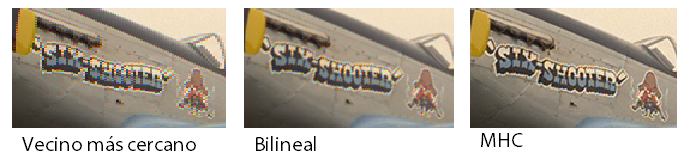
\includegraphics[scale=0.05]{imagenes/comparacion/cartel}
	\label{cartel}
  \end{center}
\end{figure}


La <<Imagen 12>> es una figura con muchas l\'ineas y dibujos con contornos. Esto se aprecia en la gran densidad que tiene la imagen que muestra las diferencias entre la imagen original y la imagen obtenida \textcolor{red}{What?} mediante el algoritmo de Vecino M\'as Cercano. Si observamos las im\'agenes obtenidas mediante la resta con sus respectivas originales se denota una gran diferencia entre el Algoritmo de Vecino M\'as Cercano y el Algoritmo de MHC.\\

Como conclusi\'on, podemos inferir que los lugares donde se muestra una variaci\'on son siempre lugares pertencientes a contornos o bordes de objetos en las im\'agenes. En cambio, en p\'ixeles sobre superficies llanas o parejas del mismo cuerpo la diferencia entre la imagen original y nuestra imagen obtenida es nula.

\newpage
\subsection{An\'alisis de tiempos}
\textcolor{blue}{Aca hay que comparar los tiempos de ejecucion entre todos los algoritmos dispuestos.}

\newpage
\section{Conclusiones y trabajo futuro}





\section{Ap\'endices}
\subsection{Ap\'endice A: Enunciado} 

%ACORDARSE DE DESCOMENTARLO%%%%%%%%%%%%%%%%%%%%%%%%%%%%%%%%%%%%%%%%%%%%%%%%%%%%%%%%%%%%%

%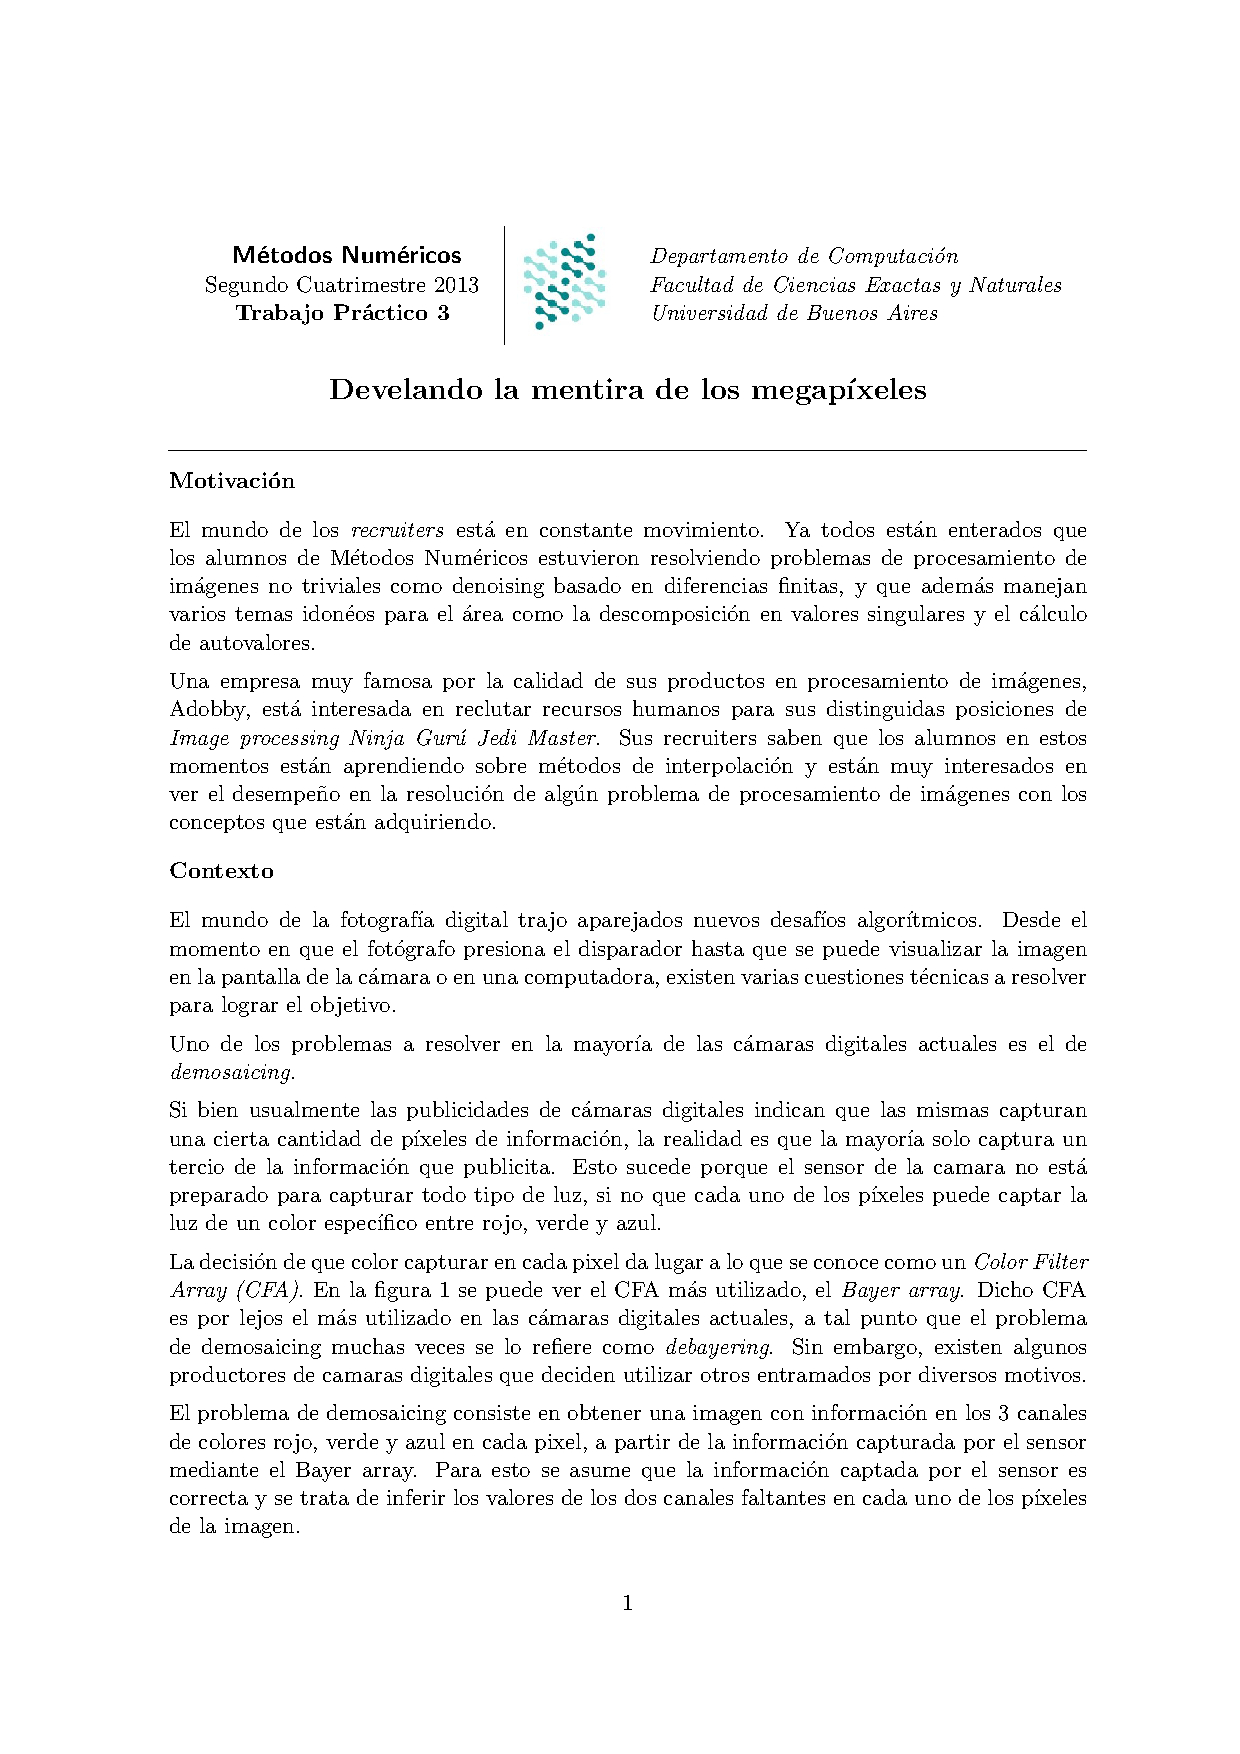
\includepdf[pages={-}]{Enunciado.pdf}

\subsection{Ap\'endice B:}
\newpage
\section{Referencias}
 
\textbf{[1]} Ron Kimmel. Demosaicing: image reconstruction from color ccd samples. \textit{IMAGE PROCESSING, IEEE TRANSACTIONS ON}, 1999. \\
\\

\textbf{[2]} Henrique S. Malvar, Li wei He, and Ross Cutler. High-quality linear interpolation for
demosaicing of bayer-patterned color images. In \textit{Proceedings of the IEEE International
Conference on Speech, Acoustics, and Signal Processing}, 2004.

\end{document}

%%%%%%%%%%%%%%%%%%%%%%%%%%%%%%%%%%%%%%%%%%%%%%%%%%%%%%%%%%%%%%%%%%%%%%%%%
\begin{figure}
  \begin{center}
	
\includegraphics[scale=0.66]{imagenes/logouba.jpg}
	\caption{Descripcion de la figura}
	\label{nombreparareferenciar}
  \end{center}
\end{figure}


\paragraph{\textbf{Titulo del parrafo} } Bla bla bla bla.
Esto se muestra en la figura~\ref{nombreparareferenciar}.



\begin{codesnippet}
\begin{verbatim}

struct Pepe {

    ...

};

\end{verbatim}
\end{codesnippet}
